%% This is the main content about this article. I should list them in an order
%% How to balance the existing model, positive and negative instance together, I shall use the dfg-method to create a dfg-matrix to incorporate the impact.
%% how to introduce them into adding long-term dependency feature. After mining the model by Inductive Miner, we have a model without long-term dependency, but we need to change the model and give the right examples.. 
%% If we change the data set, then we need to change the model into another parts, but the current methods can not solve it..
%% Should we also separate them into different sections?? Yes, we need it
%% Also, to delete the silent transition, as one option feature in our methods, we only delete it, in this situation, which will not affect the model behavoirs.

%% Or we could organize the content in this way:
%%  -- put the whole structure ahead and put all that we want to talk
%%  -- list the steps 
%%    ++ dfg-method to balance the directly-follows relation and create the corresponding directly-follows graph
%%    ++ add long-term dependency on the model
%%    ++ delete the silent transitions on the model as a post model

%% Put some words here
This chapter describes the repair algorithm to incorporate the negative instances on process enhancement. At start, the main architecture is listed to provide an overview of our strategy. Next sections will explain the main modules step by step. Firstly, the impact of the existing model, positive and negative instances are balanced in the media of the directly-follow relations. Inductive Miner is then applied to mine process models from those directly-follows relations. Again, we review the negative instances and express its impact by adding the long-term dependency. To add long-term dependency, extra places and silent transitions are created on the model, aiming to enforce the positive instances and block negative instances. Furthermore, the model in Petri net with long-term dependency can be  post-processed by reducing the silent transitions for the sake of simplicity.
\section{Architecture}
%% Describe the 
Figure \ref{fig:architecture} shows the steps of our strategy to enhance a process model. The basic inputs are an event log, and a Petri net. The traces in event log have an attribute for the classification labels of positive or negative in respect to some KPIs of business processes. The Petri net is the referenced model for the business process. To repair model with negative instances, the main steps are conducted.
\begin{figure}
	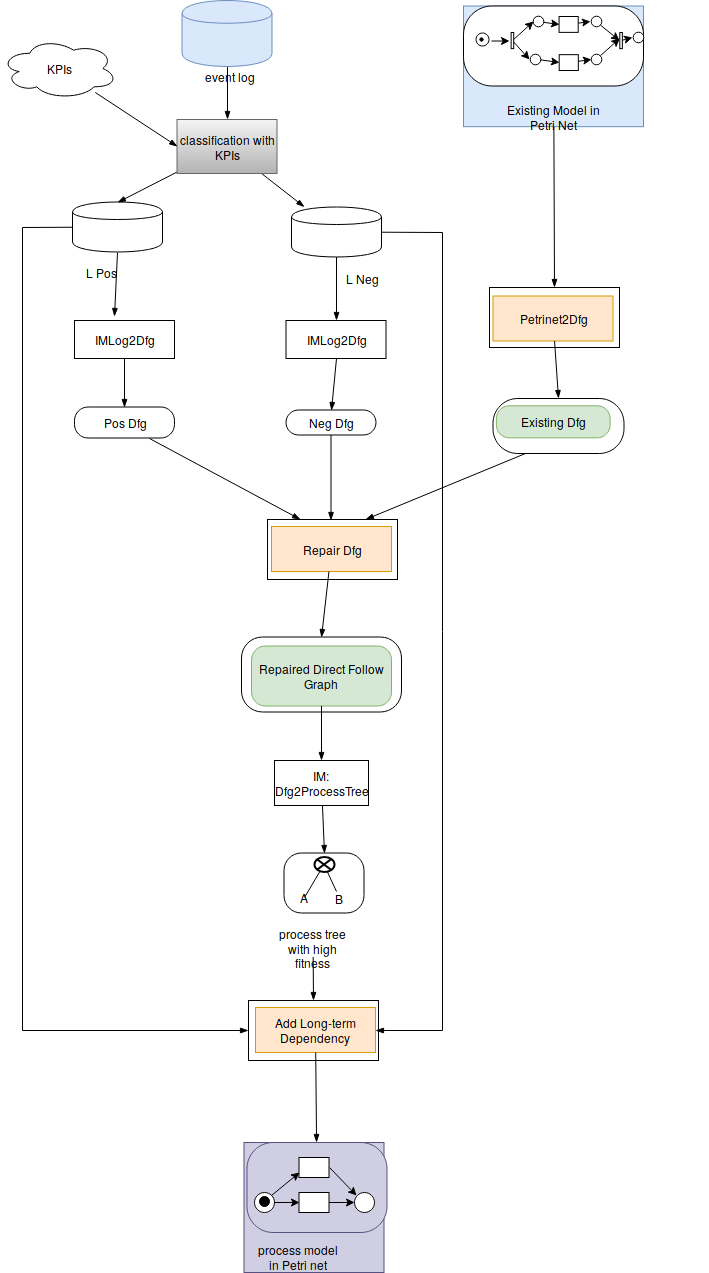
\includegraphics[width=0.9\textwidth, height=0.9\textheight]{figures/algorithm/FD_architecture_detail_02.png}
	\caption[Model Repair Architecture]{Model Repair Architecture -- \small Rectangles represents processes and output data in eclipse shape, especially customized processes and data are in doubled lattice shape. Input event log and existing model are in blue, KPIs are in cloud. The output is a petri net in purple. }
	\label{fig:architecture}
\end{figure} 
\begin{itemize}
	\item \emph{Generate directly-follows graph}\quad 
	Three directly-follows graph are generated respectively for the existing model, positive instance and negative instances from event log.
	\item \emph{Repair directly-follows graph} \quad
	The three directly-follows graphs are combined into one single directly-follows graph after balancing their impact.
	\item \emph{Mine models from directly-follows graph} \quad
	Process models are mined by Inductive Miner as intermediate results.
	\item \emph{Add long-term dependency} \quad
	Long-term dependency is detected on the intermediate models and finally added on the Petri net. To simplify the model, the reduction of silent transitions can be applied at end.
\end{itemize}
More details can be provided in the following sections.

\section{Generate directly-follows graph}
Originally, the even log $L$ is split into two sublogs, called $L_{pos}$ and $L_{neg}$. $L_{pos}$ contains the traces which is labeled as positive, while $L_{neg}$ contains the negative instances in the event log. Then, the two sublogs are passed to procedure \emph{IMLog2Dfg} to generate directly-follows graphs, respectively $G(L_{pos})$ and $G(L_{neg})$. More details about the procedure is available in \cite{leemans2013discovering}. 

To generate a directly-follows relation from  a Petri net, we gather the model behaviors by building a transitions system of its states. Then the directly-follows relations are extracted from state transitions. Based on those relations, we create a directly-follows graph for the existing model.

From the positive and negative event log, we can get the cardinality for corresponding directly-follows graph, to represent the strength of this directly-follows relation. However, when the existing model is transformed into  directly-follows graph $G(L_{ext})$, there is no point to assign cardinality on each edge. So we just set cardinality with 1 for each edge. 
\section{Repair directly-follows graph}
%% we can have subsection on it. How to repair on them??? 
To combine all information from  $G(L_{pos})$, $G(L_{neg})$ and $G(L_{ext})$, the cardinality in directly-follows graphs has to be unified into the same range. In this thesis, the unification range is [0-1], the unified value is called weight and defined as the following.
\begin{definition}[Weight of directly-follows relation]
	Given a directly-follows graph G(L), the weight of each directly-follows relation is defined as \[ Weight(E(A,B)) = \frac{Cardinality(E(A,B))}{Cardinality(E(A,*))}  \] 
	for start activities A, we have 
	\[ Weight(Start(A)) = \frac{Cardinality(Start(A))}{Cardinality(Start(*))} \]
	Similarly for end activities B, we have
	\[ Weight(End(B)) = \frac{Cardinality(End(B))}{Cardinality(End(*))} \]
	E(A,*) means all edges with source A, E(*,B) means all edges with target B, Start(*) represents all start nodes, and End(*) represents all end nodes.
\end{definition}

\section{Add long-term dependency}

\section{Reduce Silent Transitions}
